\chapter {Problem formulation in 2D space}
This chapter revolves about problem formulation in general and formulates theorem which will be the base of target research area.
A dynamic system of a unicycle is introduced and explained. World representation describes used mathematical structures. Sensor representation represents used mathematical structures to represent LiDAR point cloud.
General problem formulates theorem involving reachability and avoidance. Following different problems are interpreted and stated.

\section{Dynamic system}
The dynamic system will be used in future work to describe the dynamic and kinematic behavior of controlled plant. For future work, two kinds of the system will be used one for the 2D environment and one for the 3D environment. 2D Dynamic system will be used for concept testing, and 3D dynamic system will be used for simulations of real craft/vehicle behavior. 

\subsection{2D reference model - unicycle}
Unicycle dynamics is given by following equations:
\begin{equation} \label{eq:uni1}
    \dot{x} = v \cos \theta
\end{equation}
\begin{equation}\label{eq:uni2}
    \dot{y} = v \sin \theta
\end{equation}
\begin{equation}\label{eq:uni3}
    \dot{\theta} = \omega
\end{equation}

With defined state and input vectors:
\begin{equation}\label{eq:uni4}
x = [x, y, \theta ] 
\end{equation}
\begin{equation}\label{eq:uni5}
u(t) = [ v, \omega ]
\end{equation}

Where $x$, $y$ denotes vehicle position in euclidean space, $\theta$ denotes vehicle heading, $v$ denotes vehicle velocity and $\omega$ denotes vehicle turning rate.

\section{World representation}
The World can be represented:
\begin{enumerate}
    \item \textit {Global coordinates} - longitude,latitude and total altitude, while using Earth reference model.
    \item \textit {Local coordinates} - where where plane position is center of reference frame and point $p$ can be represented by:
    \begin{enumerate}[a.]
        \item \textit{Euclidean coordinates} - $p = [x,y,z]$, where $x$ is horizontal distance aligned to plane heading, $y$ is horizontal distance orthogonal to plane heading and $x$ is vertical distance to plane.
        \item \textit{Planar coordinates} - $p = [d, \theta, \varphi]$, where $d$ is shortest distance to plane body frame, $\theta$ is horizontal angle and $\varphi$ is horizontal angle.
    \end{enumerate}
\end{enumerate}

\textit{Global coordinates} are used for the standard representation of the world, most of the obstacle databases are working in global coordinates. Local coordinates are used for LiDAR point-cloud and surrounding world representation.


\section{General problem}
Aerial vehicle is flying in open space equipped with a LiDAR sensor on planned path given by waypoints in global coordinates:
\begin{equation}
    W_P = \left\{ w_1, w_2,w_3,\dots, w_n \right \}, n \in \N^+
\end{equation}
Where $w_1$ is starting point and $w_n$ is final point. Aerial vehicle is scanning surroundings in front of vehicle by LiDAR. Scanned cone dimensions are given by $d_L$ which is LiDAR reach distance, $\theta_L$ which is horizontal range and $\varphi_L$ which is vertical range. 

\begin{note}{Known world}
\\Know world is world known to vehicle during a flight. Vehicle known some static obstacles from common obstacle database in surroundings of route given by waypoint set $W_P$. Other source of known obstacles is given by LiDAR sensor which is capable of detecting new static and moving obstacles.
\end{note}


\begin{problem}{Optimal obstacle avoidance in restricted field of vision.} \\Aerial vehicle is defined by system dynamics $\dot{x}=f(x,u)$, where $x$ is vehicle state and $u$ is controllable input.\\
Vehicle should follow path defined by waypoints $w_i \in W_P$, vehicle have access to LiDAR sensor which can process surroundings in near real-time in cone defined by $d_l, \theta_l, \varphi_l$.\\
Vehicle must prevent crash to obstacle, by detecting possible obstacles in "known world" and executing optimal avoidance strategy.
\end{problem}

\begin{figure}[H]
    \centering
    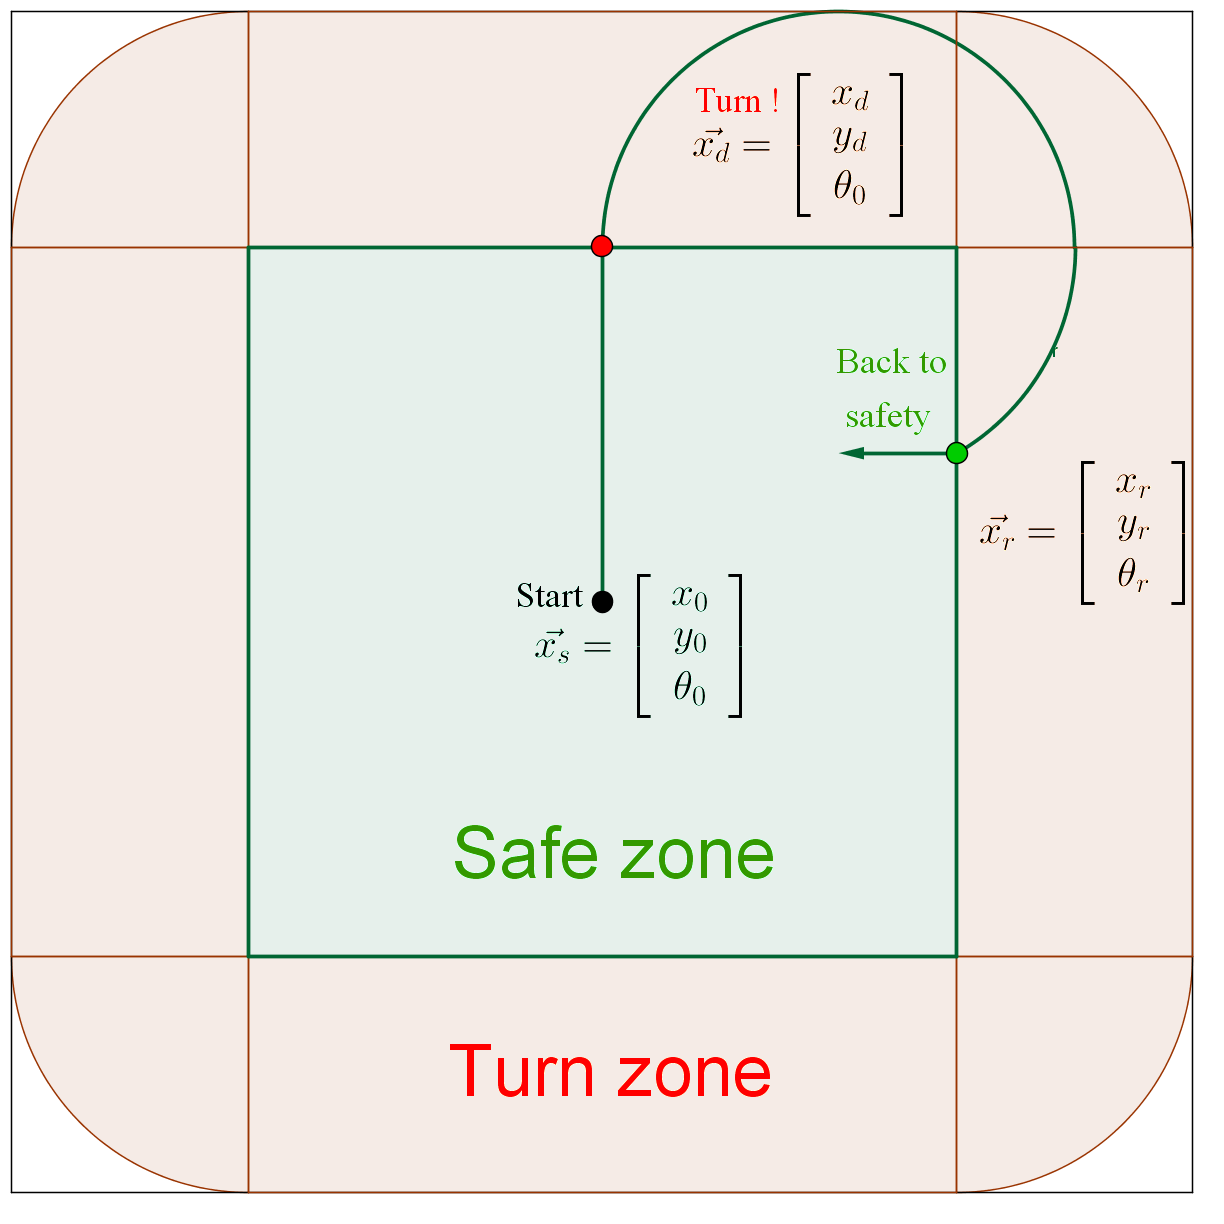
\includegraphics[width=0.5\textwidth]{\FIGDIR/01Situation.png}
    \caption{Avoid wall collision example}
    \label{fig:generalproblem}
\end{figure}

\newpage
\begin{example}{Wall avoidance for unicycle}\label{ex:avoidwallcolision}
    \\
    Unicycle is starting at start point $\vec(x_s) = [x_0, y_0, \theta_0]$ in safe zone. Control input $\vec{u} = [v, \omega]$ is not limited in safe zone, except system limitations. Unicycle reaches border between safe zone and turn zone. \\\textit{Crossing point} is dangerous, therefore is marked as $\vec{x_d} = [x_d, y_d, \theta_d]$. After crossing this point control input operations are limited only to safe operations. 
    \\\textit{Safe operations} are operations which prevent vehicle from crashing into obstacle and returns it into safe zone.
    \\When vehicle crosses border between turn zone and safe zone at return point $\vec{x_r} = [x_r, y_r, \theta_r]$, it is again safe zone, where operation set is not limited.
\end{example}

From given example \ref{ex:avoidwallcolision}., it is possible to see correlation between \textit{Safe zone} and \textit{Strong invariance} (Def. \ref{def:stronginvariance}). Nonetheless same observation can be performed between \textit{Turn zone} and \textit{Weak invariance} (Def. \ref{def:weakinvariance}). Obstacle avoidance can be divided into following problems with increasing difficulty, where simple dynamics consider operational space in 2D and complex dynamics consider operational space in 3D (tab \ref{tab:problem})
\begin{table}[H]
\centering
\begin{tabular}{|l|l||L{5cm}|c|}
\hline
Dynamics                  & Obstacle type  & Description                                     & Dificulty \\ \hline\hline
\multirow{4}{*}{Unicycle} & Convex wall    & Narrow wall in 2D                               & 1         \\ \cline{2-4} 
                          & Convex trap    & Cave formed by narrow wall  in 2D               & 2         \\ \cline{2-4} 
                          & Nonconvex wall & Rock side wall with non convex formations in 2D & 3         \\ \cline{2-4} 
                          & Nonconvex trap & Maze formed by nonconvex walls in 2D            & 4         \\ \hline
\multirow{4}{*}{Copter}   & Convex wall    &                                                 & 5         \\ \cline{2-4} 
                          & Convex trap    &                                                 & 6         \\ \cline{2-4} 
                          & Nonconvex wall &                                                 & 7         \\ \cline{2-4} 
                          & Nonconvex trap &                                                 & 8         \\ \hline
\end{tabular}
\caption{Problem with increasing difficulty definition}
\label{tab:problem}
\end{table}


